\documentclass[10pt,a4paper]{article}

\usepackage[utf8]{inputenc}
\usepackage[T1]{fontenc}
\usepackage{tgheros}
\renewcommand{\familydefault}{\sfdefault}
\usepackage{microtype}
\usepackage[margin=16mm]{geometry}
\usepackage{xcolor}
\usepackage{graphicx}
\usepackage{tabularx}
\usepackage{enumitem}
\usepackage{fontawesome5}
\usepackage{textcomp}
\usepackage{tikz}
\usepackage{eso-pic}
\usepackage[hidelinks]{hyperref}

\definecolor{navy}{HTML}{0B3A5B}
\definecolor{teal}{HTML}{1A6B7A}
\definecolor{ink}{HTML}{1C2830}
\definecolor{muted}{HTML}{5C6B73}

\pagestyle{empty}
\setlength{\parindent}{0pt}
\setlength{\parskip}{0pt}
\setlist[itemize]{leftmargin=1.15em,itemsep=4pt,topsep=5pt,parsep=0pt,partopsep=0pt}
\color{ink}
\urlstyle{same}
\frenchspacing

\newcommand{\cvsection}[1]{%
  \par\vspace{12pt}%
  {\Large\bfseries\color{navy}#1}\par\vspace{2pt}%
  {\color{teal}\rule{2.5em}{2.1pt}}\par\vspace{7pt}%
}

\newcommand{\skill}[2]{%
  \par\vspace{1pt}%
  {\bfseries\color{teal}#1}\par\vspace{1.5pt}%
  #2\par\vspace{3.5pt}%
}

\newcommand{\cventry}[3]{%
  \par\vspace{11pt}%
  \noindent\begin{tabularx}{\textwidth}{@{}>{\raggedright\arraybackslash}X >{\raggedleft\arraybackslash}p{3.7cm}@{}}
    {\large\bfseries\color{navy}#1} & {\color{muted}#2}\\[0.28em]
    \multicolumn{2}{@{}>{\raggedright\arraybackslash}p{\dimexpr\textwidth}@{}}{\color{teal}#3}\\
  \end{tabularx}\par\vspace{3pt}%
}

\newcommand{\eduitem}[4]{%
  \par\vspace{8pt}%
  \noindent\begin{tabularx}{\textwidth}{@{}>{\raggedright\arraybackslash}X >{\raggedleft\arraybackslash}p{3.7cm}@{}}
    \textbf{#1} & {\color{muted}#2}\\[0.15em]
    #3 & #4\\
  \end{tabularx}%
}

\newcommand{\cvphoto}{%
  \begin{tikzpicture}
    \begin{scope}
      \clip[rounded corners=1.8mm] (0,0) rectangle (32mm,32mm);
      \node[inner sep=0pt, anchor=north west] at (0,32mm) {%
        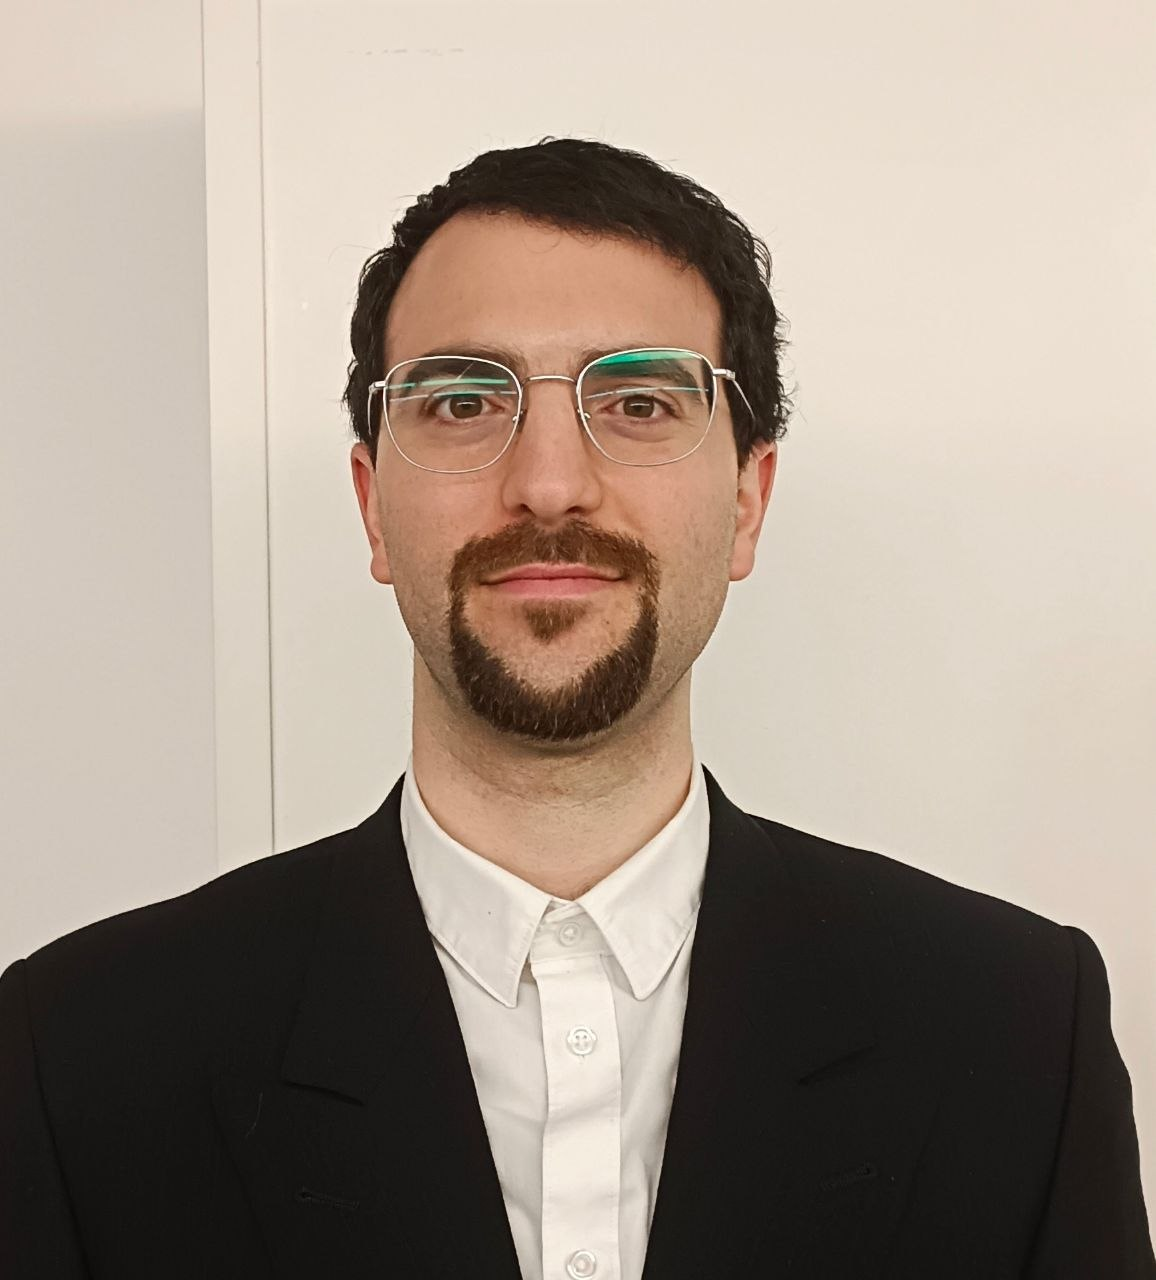
\includegraphics[width=32mm]{photo_2.jpg}%
      };
    \end{scope}
  \end{tikzpicture}%
}

\hypersetup{
  pdftitle={Gianluigi Sabatino -- Laboratory Technician},
  pdfauthor={Gianluigi Sabatino}
}


% Codice QR: pagina 2, in basso a destra (allineato ai margini di 16 mm)
\newcommand{\qrsize}{22mm}
\AddToShipoutPictureFG{%
  \ifnum\value{page}=2
    \AtPageLowerLeft{%
      \put(\LenToUnit{\dimexpr\paperwidth-16mm-\qrsize\relax},\LenToUnit{16mm}){%
        
\includegraphics[width=\qrsize]{QRcurriculum.jpg}%
      }%
    }%
  \fi
}

\begin{document}
\fontsize{10}{13.4}\selectfont

\noindent
\begin{minipage}[t]{\dimexpr\textwidth-36mm\relax}
  \vspace{0pt}%
  {\fontsize{26}{28}\selectfont\bfseries\color{navy} Gianluigi Sabatino, M.Sc.}\\[0.45em]
  {\fontsize{12}{14}\selectfont\color{teal} Laboratory Technician\enspace\textbar\enspace Biologist}\\[0.7em]
  {\color{muted}\small
    \faIcon{map-marker-alt}\enspace Elisenstra{\ss}e 1, 1230 Vienna, Austria
    \enspace\textperiodcentered\enspace
    \faIcon{phone}\enspace +43 660 9673179\\[0.28em]
    \faIcon{envelope}\enspace \href{mailto:gianluigi.sabatino94@gmail.com}{gianluigi.sabatino94@gmail.com}
    \enspace\textperiodcentered\enspace
    \faIcon{linkedin}\enspace \href{https://www.linkedin.com/in/gianluigi-sabatino/}{linkedin.com/in/gianluigi-sabatino}%
  }
\end{minipage}\hfill
\begin{minipage}[t]{32mm}
  \vspace{0pt}%
  \raggedleft\cvphoto
\end{minipage}

\vspace{11pt}
{\color{teal!70}\rule{\textwidth}{0.6pt}}

\cvsection{Profile}
Biologist specialized in laboratory techniques, with research experience in analytical chemistry and polymer characterization. Over two years of HPLC analysis and method development (October 2021--May 2022 and September 2024--January 2026). Day-to-day work includes calibration, maintenance and sterilization of equipment, plus MALDI-TOF mass spectrometry, NMR, molecular biology, cell culture and histology at TU Wien and the Medical University of Vienna.

\cvsection{Laboratory skills}
\skill{Analytical}{Spectroscopy (UV, VIS, IR); HPLC (UV, FL, ELSD; HILIC and reverse phase); MALDI-TOF mass spectrometry; NMR; titrations; GPC.}
\skill{Molecular biology}{Protein purification and characterization; DNA/RNA extraction and characterization; gel electrophoresis; RT-PCR; genomic sequencing (Illumina MiSeq).}
\skill{Cell culture}{Prokaryotic and eukaryotic cultures; selection of prokaryotic strains; propagation of cell lines; transformation; administration of molecules.}
\skill{In vivo}{Blood, tissue/organ and bronchoalveolar sampling; intraperitoneal, intravenous, intramuscular and subcutaneous injection; inhaled dosing; anesthesia; unrestrained whole-body plethysmography; euthanasia; dissection.}
\skill{Histology}{Organ dissection, fixation and staining; histological preparations; microscopy (TissueFAX).}
\skill{Data}{Statistical analysis and bioinformatics; mass-spectrum analysis; R, Python, GraphPad Prism, MassHunter, \mbox{MestReNova}, mMass, BWA, MEGA-X, BLAST.}
\skill{GMP}{Familiar with GMP.}

\cvsection{Experience}
\cventry{Laboratory Technician}{Sep 2024 -- Jan 2026}{Institute of Applied Synthetic Chemistry, TU Wien --- Macromolecular Chemistry}
{\small\color{muted} WWTF project ``Exploring the Glycome: Identifying Glycosylation-Related Biomarkers for severity stratification in Chronic Fatigue Syndrome'' (\texteuro 99,946).}\par
\begin{itemize}
  \item \parbox[t]{\linewidth}{Established a biomarker-discovery pipeline for ME/CFS severity stratification on 150+ blood and milk samples, using MALDI-TOF mass spectrometry and HILIC/RP-HPLC with fluorescence detection to identify glycosylation patterns as inflammatory indicators.}
  \item \parbox[t]{\linewidth}{Optimized fluorescent glycan conjugation for reproducible O-glycosylation, N-glycosylation and sialic acid analysis in complex biological matrices, generating datasets on glycocalyx damage markers.}
  \item \parbox[t]{\linewidth}{With the MedUni Wien immunology team, correlated hypo-glycosylation biomarkers with pro-inflammatory immune activation in post-infectious chronic fatigue.}
  \item \parbox[t]{\linewidth}{Poster at the AustroCarb workshop, Vienna, 14 February 2025: ``N-glycan profiles of cells cultured with diverse monosaccharide treatments''.}
  \item \parbox[t]{\linewidth}{Parallel project (5 months): synthesized and characterized acrylate-based hydrogels for biomedical applications, including thermal- and photo-initiated free-radical polymerization (NMR and refractive-index analysis).}
  \item \parbox[t]{\linewidth}{Prepared laboratory-course materials and supported the public outreach event The Long Night of Research.}
\end{itemize}

\cventry{Research Intern}{May 2024 -- Aug 2024}{Department of Pathophysiology and Allergy Research, Medical University of Vienna}
\begin{itemize}
  \item \parbox[t]{\linewidth}{Preclinical work toward humanized mouse models: mast-cell degranulation (Evans blue), isolation of cells from murine bone marrow and spleen, colorimetric assays, PBMC isolation by Ficoll density-gradient centrifugation, and multiparameter flow cytometry.}
  \item \parbox[t]{\linewidth}{Animal experimentation under Austrian welfare regulations: injection routes (IP/IV/IM/SC), anesthesia, tissue harvesting and ethical euthanasia.}
\end{itemize}

\cventry{Research Intern}{Oct 2021 -- May 2022}{Institute of Applied Synthetic Chemistry, TU Wien}
\begin{itemize}
  \item \parbox[t]{\linewidth}{Developed an HPLC method for sialic acid quantification in dairy products.}
  \item \parbox[t]{\linewidth}{Synthesized superabsorbent polymers for biomedical applications, and characterized polymer molecular weight by GPC.}
\end{itemize}

\cvsection{Education}
\eduitem{Master's degree in Functional Genomics}{2017--2019}{University of Trieste}{104/110}
\eduitem{Bachelor's degree in Biological Sciences and Technologies}{2013--2016}{University of Trieste}{110/110}
\eduitem{Diploma in Chemical Engineering}{2008--2013}{Technical-industrial high school G.\ D'Annunzio -- M.\ Fabiani}{91/100}

\cvsection{Languages and other}
\noindent
\begin{minipage}[t]{0.60\textwidth}
  \vspace{0pt}%
  Italian, native\\[0.38em]
  English, full professional proficiency\\[0.38em]
  German, B1 (professional working proficiency)\\[0.38em]
  Greek, basic
\end{minipage}\hfill
\begin{minipage}[t]{0.34\textwidth}
  \vspace{0pt}%
  Born 6 May 1994\\[0.38em]
  Italian\\[0.38em]
  Driving licence B\\[0.38em]
  Guitar and cooking.
\end{minipage}

\end{document}
